\documentclass[journal]{vgtc}                     % final (journal style)
%\documentclass[journal,hideappendix]{vgtc}        % final (journal style) without appendices
%\documentclass[review,journal]{vgtc}              % review (journal style)
%\documentclass[review,journal,hideappendix]{vgtc} % review (journal style)
%\documentclass[widereview]{vgtc}                  % wide-spaced review
%\documentclass[preprint,journal]{vgtc}            % preprint (journal style)


%% Uncomment one of the lines above depending on where your paper is
%% in the conference process. ``review'' and ``widereview'' are for review
%% submission, ``preprint'' is for pre-publication in an open access repository,
%% and the final version doesn't use a specific qualifier.

%% If you are submitting a paper to a conference for review with a double
%% blind reviewing process, please use one of the ``review'' options and replace the value ``0'' below with your
%% OnlineID. Otherwise, you may safely leave it at ``0''.
\onlineid{0}

%% In preprint mode you may define your own headline. If not, the default IEEE copyright message will appear in preprint mode.
%\preprinttext{To appear in IEEE Transactions on Visualization and Computer Graphics.}

%% In preprint mode, this adds a link to the version of the paper on IEEEXplore
%% Uncomment this line when you produce a preprint version of the article 
%% after the article receives a DOI for the paper from IEEE
%\ieeedoi{xx.xxxx/TVCG.201x.xxxxxxx}

%% declare the category of your paper, only shown in review mode
\vgtccategory{Research}

%% please declare the paper type of your paper to help reviewers, only shown in review mode
%% choices:
%% * algorithm/technique
%% * application/design study
%% * evaluation
%% * system
%% * theory/model
\vgtcpapertype{please specify}

%% Paper title.
\title{Task-dependent utility of differentially private scatterplots through Scagnostics}

%% Author ORCID IDs should be specified using \authororcid like below inside
%% of the \author command. ORCID IDs can be registered at https://orcid.org/.
%% Include only the 16-digit dashed ID.
\author{%
  \authororcid{Harith Rathish}{0000-0002-1452-1814},and 
  \authororcid{Hans-Jörg Schulz}{0000-0001-9974-535X}
}

\authorfooter{
  %% insert punctuation at end of each item
  \item
  	Harith Rathish is with Aarhus University.
  	E-mail: harith@cs.au.dk

  \item Panagiotis Karras is with Aarhus University.
  	E-mail: piekarras@gmail.com
   
  \item
  	Hans-Jörg Schulz is with Aarhus University
        E-mail: hjschulz@cs.au.dk
}

%% Abstract section.
\abstract{Private and sensitive data has been increasingly the subject of visual analysis tasks. Data owners increasingly use differential privacy to enable public data sharing with a guaranteed amount of privacy. Balancing the need to prevent privacy leaks with that of getting meaningful insights from the data is challenging. While the visual output of differentially private data is affected by algorithm choice, privacy level and binning sizes, there is a lack of guidance on choosing and balancing the effect of these parameters. Such guidance needs a metric of how much visual utility is preserved by the privatization. This project explores how scagnostics can be used as a visual utility metric for differentially private scatterplots. We provide scagnostics data from 560 differentially private scatterplots and a user interface for exploring the parameter space of differential privacy and how it affects the scagnostics.  % % filler text. Replace with your abstract.
  %
  %% We recommend that you link to your supplemental material here in the abstract, as well
  %% as in the Supplemental Materials section at the end.
  A free copy of this paper and all supplemental materials are available at \url{https://osf.io/xykef/}.
}

%% Keywords that describe your work. Will show as 'Index Terms' in journal
%% please capitalize first letter and insert punctuation after last keyword
\keywords{Radiosity, global illumination, constant time}

%% A teaser figure can be included as follows
\teaser{
  \centering
  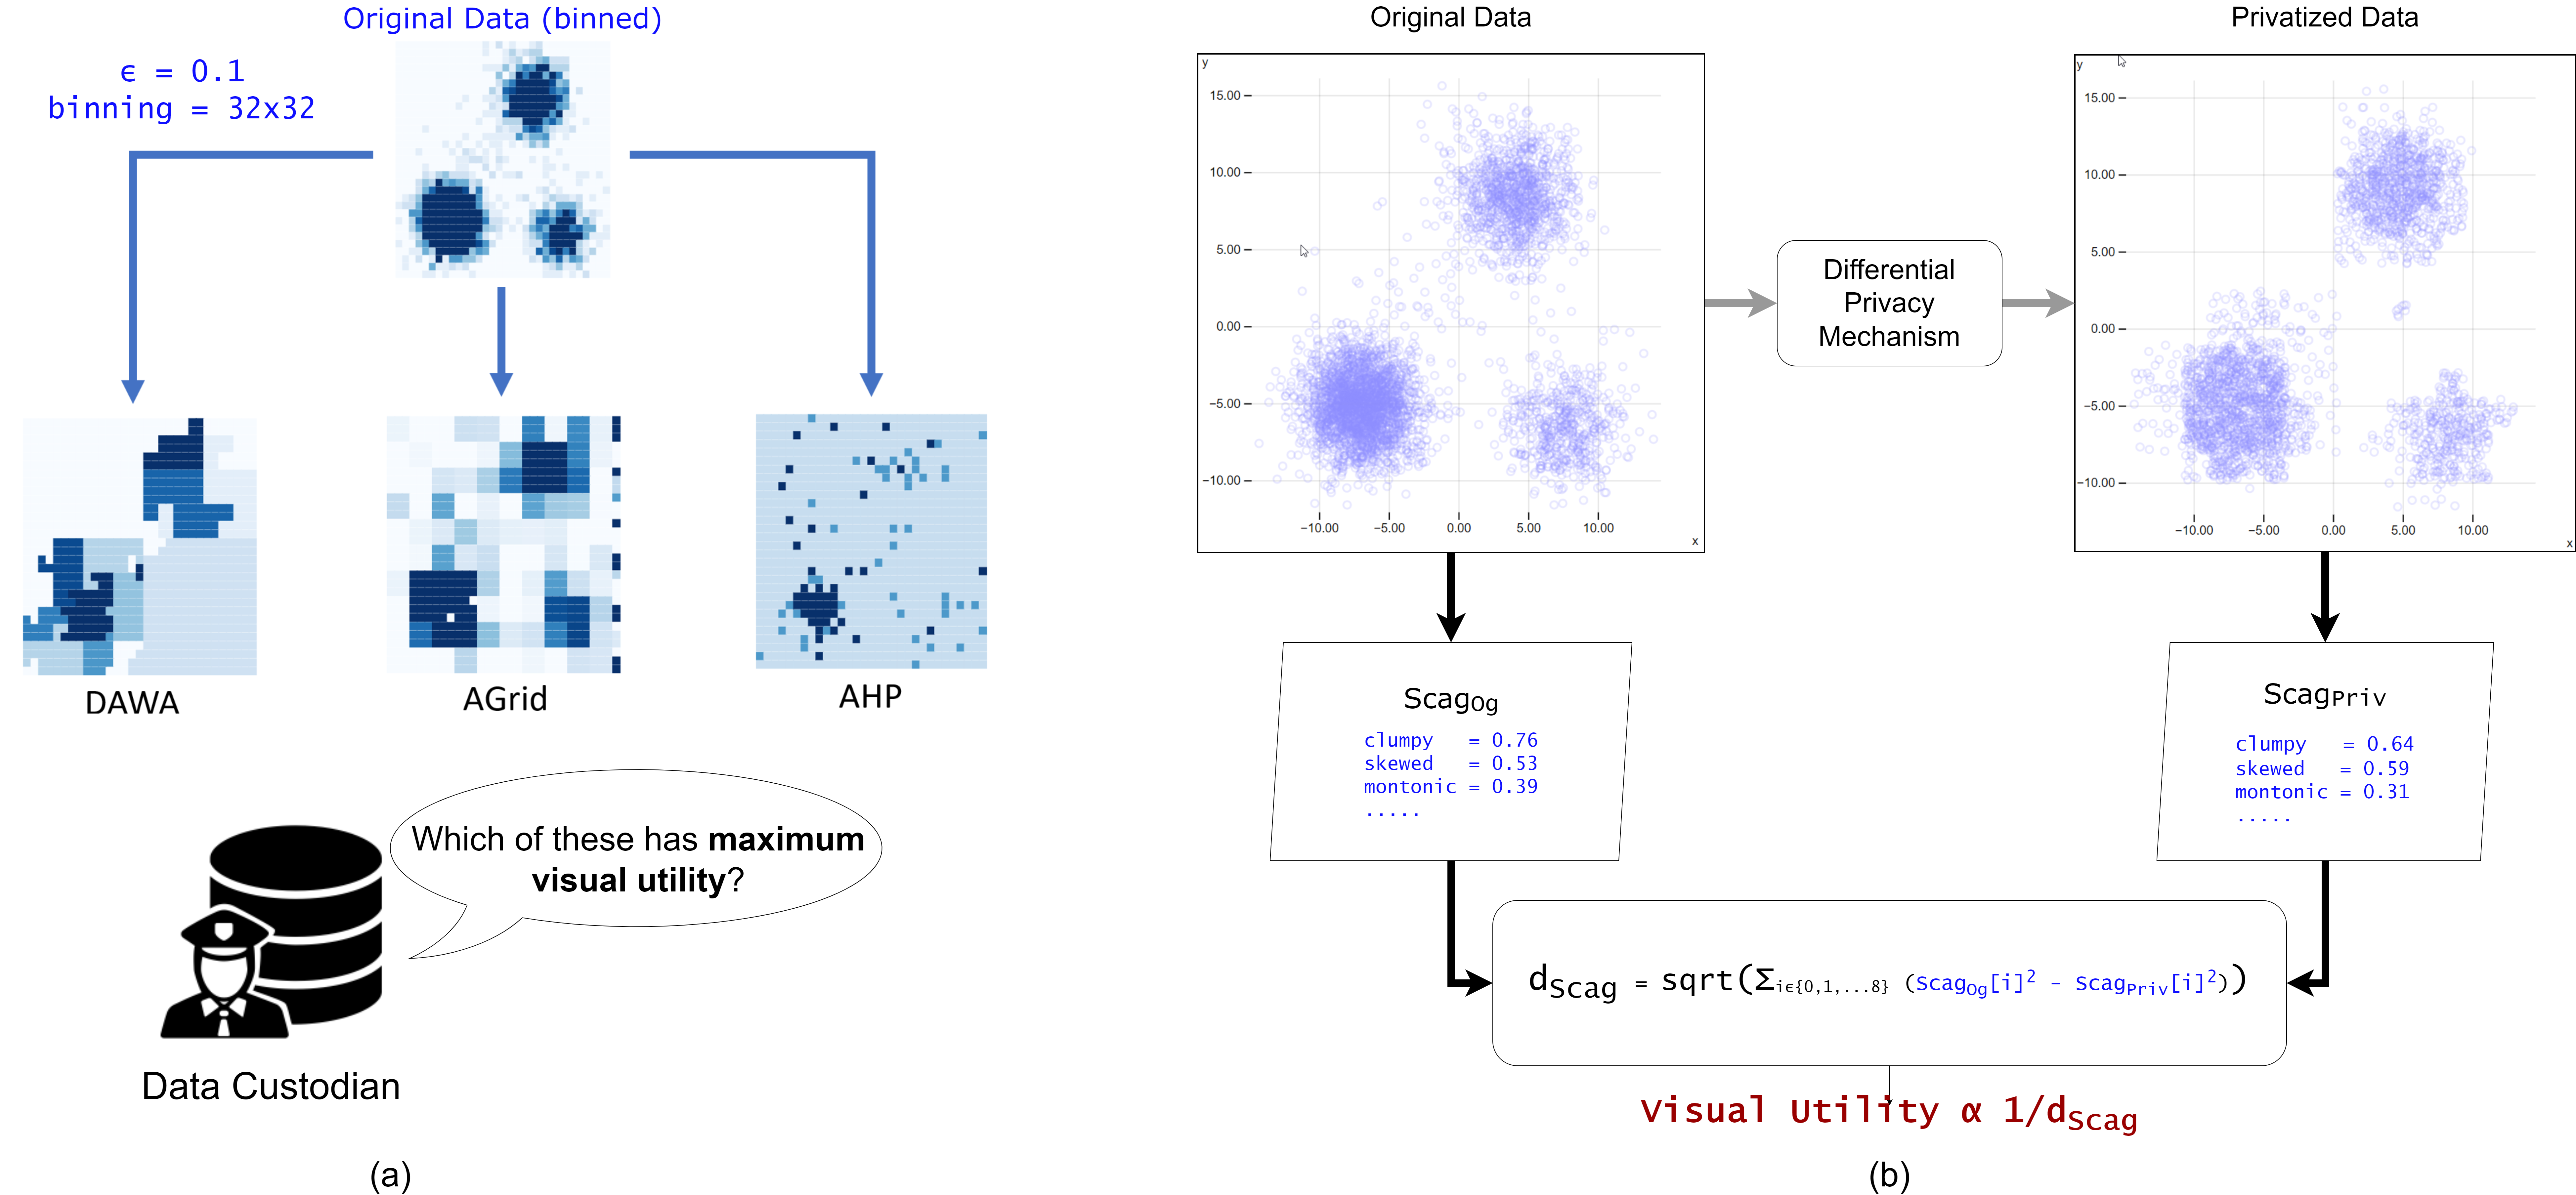
\includegraphics[width=1.05\linewidth]{figs/new_teaser.png}
  \caption{%
  	Overview of the need for a visual utility metric in differential privacy and the proposed solution using scagnostics . (a) Privatizing the original data with different DP mechanisms (DAWA, AGrid, and AHP) produce different looking outputs
   % , despite the parameters $\epsilon = 0.1$ and $binning = 32x32$ being the same. To choose between these outputs, data custodians need a reliable metric of visual utility. 
   (b) Computing visual utility by taking the Euclidean distance between the scagnostics vectors of the original and private data.
   % The scagnostics vectors of the original and private data are denoted as $Scag_{Og}$ and $Scag_{Priv}$, respectively. We consider visual utility inversely proportional to the \textbf{Euclidean distance $d_{Scag}$} between $Scag_{Og}$ and $Scag_{Priv}$.%
  }
  \label{fig:teaser}
}

%% Uncomment below to disable the manuscript note
%\renewcommand{\manuscriptnotetxt}{}

%% Copyright space is enabled by default as required by guidelines.
%% It is disabled by the 'review' option or via the following command:
%\nocopyrightspace


%%%%%%%%%%%%%%%%%%%%%%%%%%%%%%%%%%%%%%%%%%%%%%%%%%%%%%%%%%%%%%%%
%%%%%%%%%%%%%%%%%%%%%% LOAD PACKAGES %%%%%%%%%%%%%%%%%%%%%%%%%%%
%%%%%%%%%%%%%%%%%%%%%%%%%%%%%%%%%%%%%%%%%%%%%%%%%%%%%%%%%%%%%%%%

%% Tell graphicx where to find files for figures when calling \includegraphics.
%% Note that due to the \DeclareGraphicsExtensions{} call it is no longer necessary
%% to provide the the path and extension of a graphics file:
%% 
\includegraphics{diamondrule} is completely sufficient.
\graphicspath{{figs/}{figures/}{pictures/}{images/}{./}} % where to search for the images

%% Only used in the template examples. You can remove these lines.
\usepackage{tabu}                      % only used for the table example
\usepackage{booktabs}                  % only used for the table example
\usepackage{lipsum}                    % used to generate placeholder text
\usepackage{mwe}                       % used to generate placeholder figures

%% We encourage the use of mathptmx for consistent usage of times font
%% throughout the proceedings. However, if you encounter conflicts
%% with other math-related packages, you may want to disable it.
\usepackage{mathptmx}                  % use matching math font

\begin{document}

%%%%%%%%%%%%%%%%%%%%%%%%%%%%%%%%%%%%%%%%%%%%%%%%%%%%%%%%%%%%%%%%
%%%%%%%%%%%%%%%%%%%%%% START OF THE PAPER %%%%%%%%%%%%%%%%%%%%%%
%%%%%%%%%%%%%%%%%%%%%%%%%%%%%%%%%%%%%%%%%%%%%%%%%%%%%%%%%%%%%%%%

%% The ``\maketitle'' command must be the first command after the
%% ``\begin{document}'' command. It prepares and prints the title block.
%% the only exception to this rule is the \firstsection command
\firstsection{Introduction}

\maketitle

%% \section{Introduction} %for journal use above \firstsection{..} instead
Differential privacy~\cite{Dwork2006} mechanisms are an invaluable tool in privacy-preserving data analysis and visualization~\cite{Bhattacharjee2020}.
By adding noise to the original data, they can protect sensitive data records (e.g., patient data) while still allowing analysts to derive analytical insight from them.
The amount of noise added governs the balance between privacy and utility inherent in this mechanism: The more noise, the higher the privacy guarantees, but the lower the remaining utility of the data -- and vice versa.

Finding a suitable trade-off between privacy and utility is not an easy task.
In differential privacy, the parameter $\epsilon$ is key to controlling the privacy guarantees, and thus, in turn, also the remaining accuracy of the data and thereby their usefulness for analyses.
However, even for the same value of $\epsilon$, different privacy mechanisms produce different outputs with different utility for their visual analysis~\cite{Panavas2022}.
This is illustrated in Fig.~\ref{fig:teaser} (a). In this example, an analyst can have different conclusions about the number of clusters in the data depending on which output they look at.


%For example, consider the binned scatterplot in Figure \ref{fig:the_problem}, labelled "Original Data" and with 32x32 bins. The darker the colour of a bin, the more the number of points within the bin. Suppose that we want to privatize this using an $\epsilon$ value of $0.5$. Below the original data are outputs of three differential privacy mechanisms, run with the same parameters. Notice how different they look from the original data, as well as among themselves. While all three clusters are preserved by AGrid, only two clusters are preserved by DAWA and only one by AHP. Thus, an analyst whose task is to identify clusters \cite{Sarikaya2018} would draw different conclusions from these plots. Out of these, we can visually perceive that the AGrid plot preserves the "overall" structure of the original data. But how can we quantify the extent of this preservation?

Thus, while the statistical privacy guarantees are quantifiable and steerable via the $\epsilon$ parameter, the utility of the visual output is not.
The reason is that utility can hardly be assessed in all generality. It must considered in the context of the analysis task to be performed, as a differential privacy mechanism may preserve some patterns in the data but not others.
For computational analyses, that usually means to run the analysis algorithm on both -- the original and the private data -- and to measure their discrepancy~\cite{Karr2006}.


Yet, for visual-interactive analyses, such a comparison of original and private visualization is not as straightforward.
While a pixel-by-pixel comparison of two output visualizations is certainly possible, the result does not capture whether the private visualization is or is not showing a sought pattern in the data, as shown in Figure ~\ref{fig:pixel_by_pixel_is_meh}.

\begin{figure}[h]
  \centering
    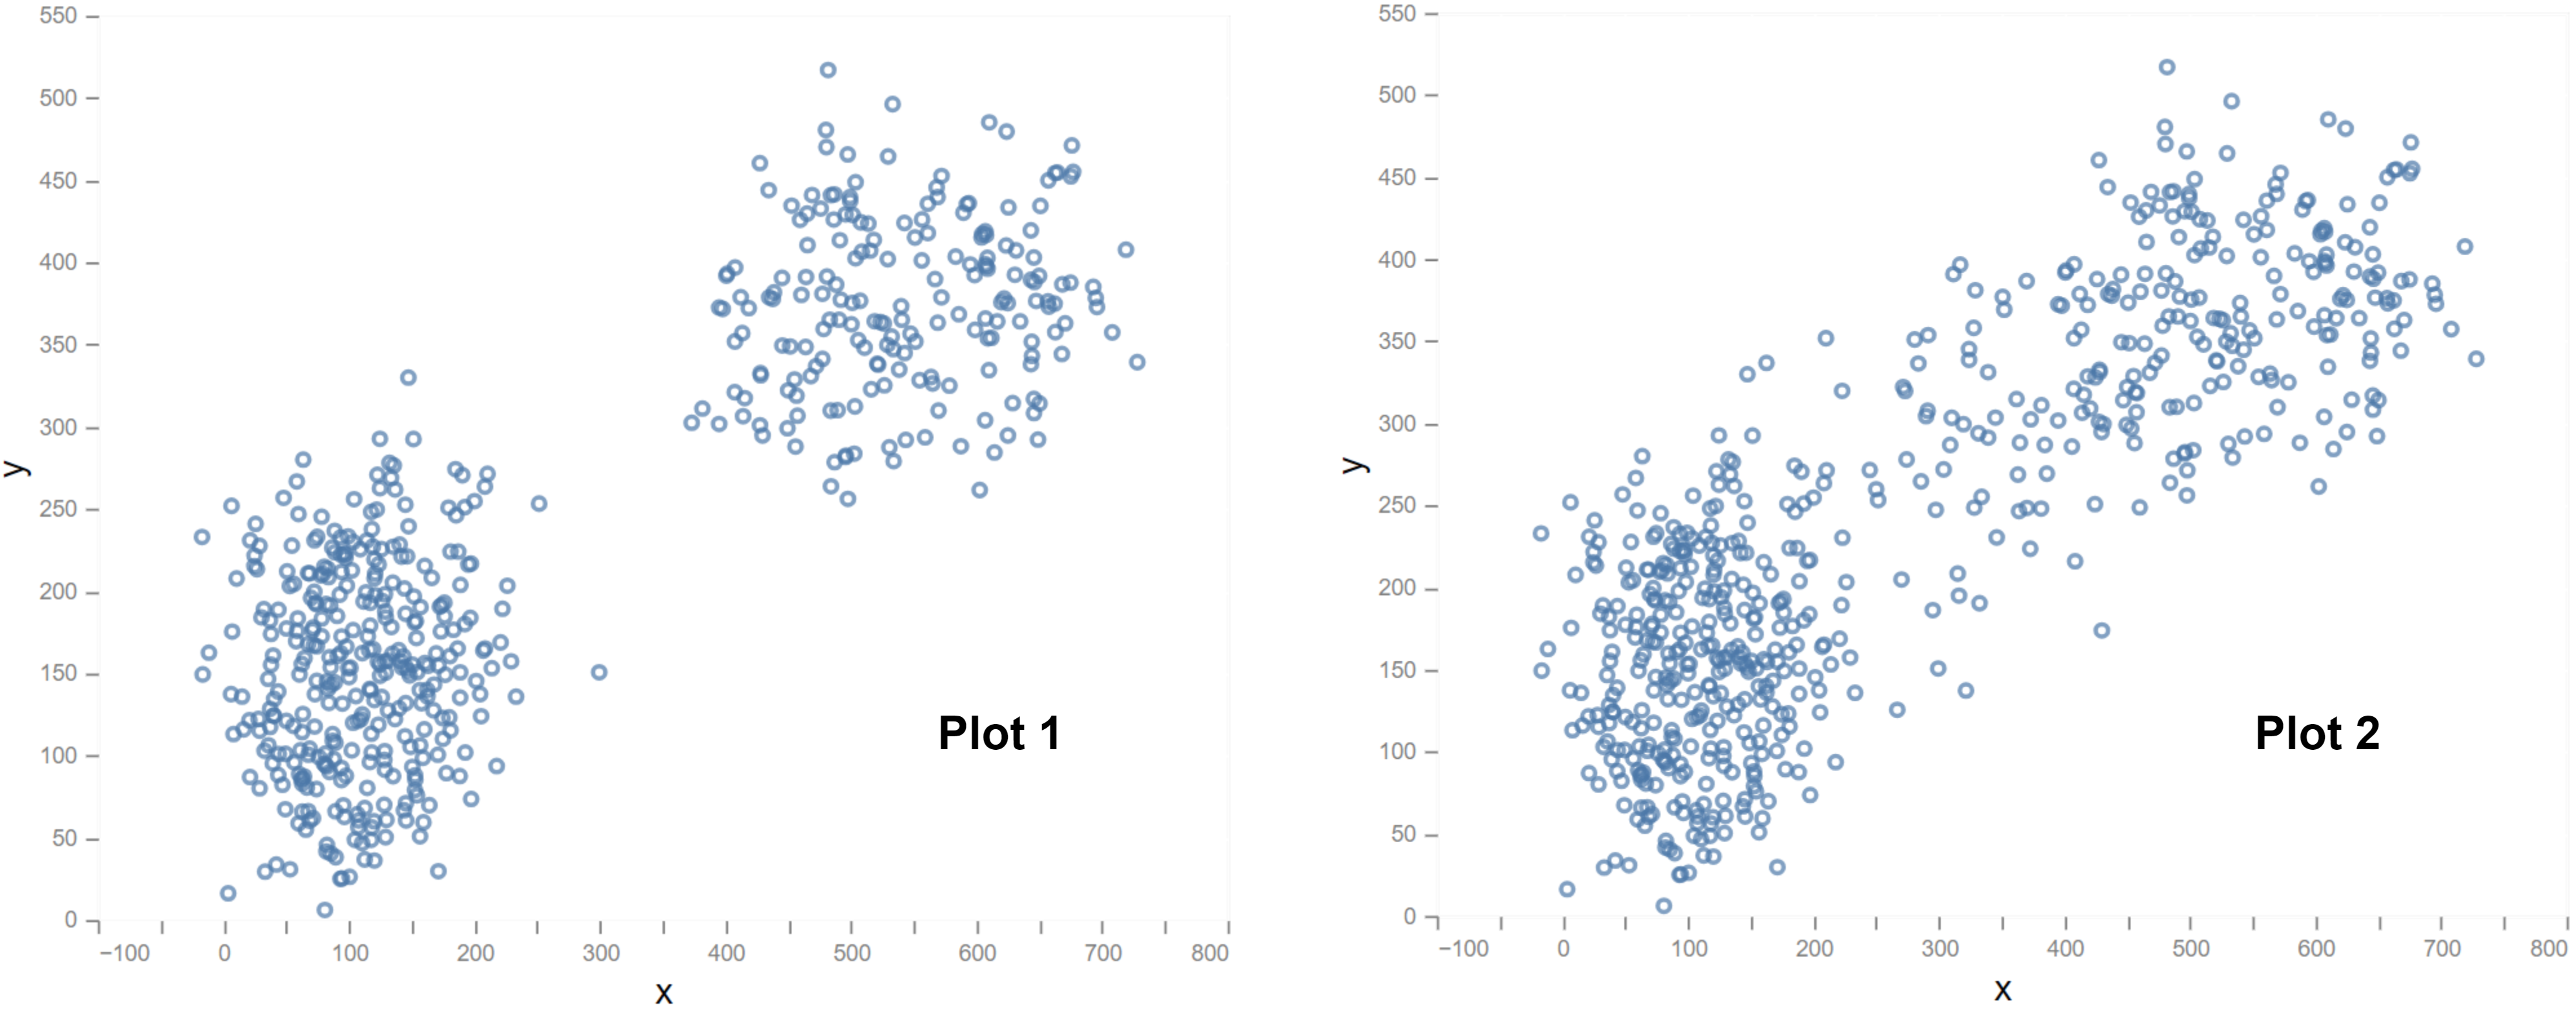
\includegraphics[width=0.49\textwidth]{figs/pixel_by_pixel_is_meh.png}
  
  \caption{Plot 2 was made by adding points between the two clusters shown on plot 1. While plot 1 clearly shows a clustered pattern, plot 2 suggests a correlation between x and y. While a pixel-by-pixel comparison would suggest these plots are different, it would not suggest that plot 2 now displays a correlation pattern. }
  \label{fig:pixel_by_pixel_is_meh}
\end{figure}

This is where our approach comes in: Instead of comparing the images, we numerically capture their appearance and compare those numbers with each other.
In this paper, we use scatterplots as the visualizations in question and Scagnostics~\cite{Wilkinson2005} as the means to capture their appearance.
Depending on the task, we then select suitable Scagnostics measures that we aim to preserve as best as possible in the private scatterplots.
For example, for a clustering/grouping task, it makes sense to preserve the \emph{clumpiness} measure of the plot, as we are first and foremost interested in the plot's dense areas.
Whereas for a correlation task, we would be more interested in preserving its \emph{stringiness} measure, as we are mainly interested in any bands appearing in the plot.

%The notion of data utility does not only appear in the context of privacy-preserving techniques, but is also used to assess data reduction and compression techniques, as well as for synthetic datasets.

As a result of this approach, we can choose an appropriate differential privacy methods and fine-tune its parameter $\epsilon$ to preserve exactly those visual features needed for the analysis task at hand.
By extending our approach from individual scatterplots to scatterplot matrices, we can also negotiate utility tradeoffs between different variables by choosing a different $\epsilon$ for them.

In summary, we contribute:
\begin{itemize}
\item Data on the performance of scagnostics as a task-based utility metric for differentially private scatterplots.
\item An open-source implementation of our approach that can be used for exploring the parameter space of differential privacy and how it affects the scagnostics of the data.
\item A usage example of our approach for a real-world use case [ADD DETAILS].
\end{itemize}

%We need a different metric to quantify the visual utility of these plots. This metric addresses the following question - how well can a visualization task be performed on the privatized output? For example, in Figure \ref{fig:the_problem}, for the task of identifying clusters, this metric should indicate the extent to which the clusters are preserved. Such a metric would help data curators choose the value of $\epsilon$ with an algorithm that both preserves privacy and lets analysts perform visualization tasks. 
        
%While the choice among the three plots shown in Figure \ref{fig:the_problem} may seem straightforward, the number of possibilities increases with the number of algorithms, possible $\epsilon$ values and binning modes. Choosing which of these numerous outputs is best for visualization tasks requires a quantifiable measure. In this paper, we propose a system to explore the parameter space of differential privacy using Scagnostics \cite{Wilkinson2005}.  

%Scagnostics is a set of statistical measures that quantify the appearance of a scatterplot. It provides metrics for identifying correlations and patterns in two-dimensional data, including features described as shape, trend, and coherence. Comparing these measures for both the original data and the privatized data can show how much they differ from one another. The larger this difference, the easier or harder it is to perform visualization tasks. We hypothesize that the visual utility of the privatized  plot is proportional to the difference in the scagnostics measures.

%With this hypothesis in mind, we have developed a system that aims to help data curators explore the parameter space of differential privacy and decide which combination of parameters is best for preserving the plot's appearance. We also tested this idea on artificially generated datasets and have provided preliminary benchmarks of the effectiveness of scagnostics. We will also show how well this measure coincides with users' perception of utility using \cite{Panavas2022} et al.'s user evaluation of utility for differentially private scatterplots, which will be discussed further in related work. \textcolor{red} {\textit{@TODO: Talk about the sensitivity of scagnostics and that we used a denoising mechanism?}}
    
    
% \begin{itemize}
%     \item Our focus: Measuring utility for differentially private scatterplots
%     \item Our perspective on utility: How does the plot aid the ability to do tasks?
%     \item Tasks for scatterplots: identifying clusters, trends etc. rely on maintaining the distribution of the data even when adding noise
%     \item To make sure the dist. is maintained, we have to measure it : Scagnostics!
%     \item Idea: Use the difference in Scagnostics measures as a proxy for utility. Which measures depend on which tasks the analyst wants to do.
%     \item Evaluation: Match benchmark metrics against existing pilot study on utility. See if they coincide or not
%     \item 
% \end{itemize}


\section{Related Work}
Measuring the utility of privatized data is a tough task. There is no accepted utility measure that works for all contexts of use, as shown by Bertino et al. \cite{Bertino2008}. That being said, there are a few different contexts in which utility was measured in the privacy-preserving visualization domain. Dasgupta et al. \cite{Dasgupta2013} proposed utility metrics designed using the visual uncertainty framework. However, these metrics were made for k-anonymity-based privatization methods and don't translate well to differential privacy.

Apart from a quantitative approach, Pavas et. al. \cite{Panavas2022} evaluated the utility of five DP mechanisms through a user study. Participants were asked to rate how well these mechanisms preserve three characteristic features of a binned scatterplot - clusters, correlations and distributions. This produced a ranking of the mechanisms according to their utility, and in our paper, we aim to augment these findings with a task-based quantitative measure of utility.

\textit{\textcolor{red}{Panavas's poster discusses three features, but what if the data doesn't align with any of these? Is our method \textbf{feature agnostic?} i.e. Would it matter if it's 
 a cluster/correlation/anything else we want to preserve? Would scagnostics capture everything? But then, would a task-based approach still work because it's based on distribution characteristics? TBD after results. }}

% \begin{itemize}
%     \item Utility in the context of privacy-preserving vis
%     \begin{itemize}
%         \item How useful a privatized output is = how close to the original data it is
%     \end{itemize}
%     \item Measuring utility for privacy-preserving vis - Dasgupta et al. \cite{Dasgupta2013}
%     \begin{itemize}
%         \item Focused on vis privatized with k-anonymization methods
%         \item Overlaps, uncertainty metrics etc.
%         \item Gap: Didn't focus on differential privacy. Diff privacy is often superior to anonymization techniques
%     \end{itemize}
%     \item Existing work on diff priv for vis - Panavas et al. \cite{Panavas2022}
%     \begin{itemize}
%         \item Did a pilot study for diff priv scatterplots
%         \item found some preliminary results
%         \item Gap : Their study asked if the noisy plot "preserves" clusters, correlations, and trends and had a qualitative scale. This is subjective to the user. Our approach will give a quantitative measure on how much it actually preserves. 
%     \end{itemize}
    
% \end{itemize}

\section{Overview}

Scagnostics \cite{Wilkinson2005} is a set of nine measures for characterising scatterplots; see Figure \ref{fig:scag_overview}. The computation of visual utility using Scagnostics is shown in Figure \ref{fig:teaser} (b). We take the original and the privatized versions of the data and compute their Scagnostics vectors $Scag_{Og}$ and $Scag_{priv}$, respectively. These are 9-dimensional vectors where $Scag[i]_{Og}$ and $Scag[i]_{Priv}$ represent individual scagnostics measures, such as clumpiness, skewdness etc.

\begin{figure}[tbp]% specify a combination of t, b, p, or h for top, bottom, on its own page, or here
  \centering % avoid the use of \begin{center}...\end{center} and use \centering instead (more compact)
  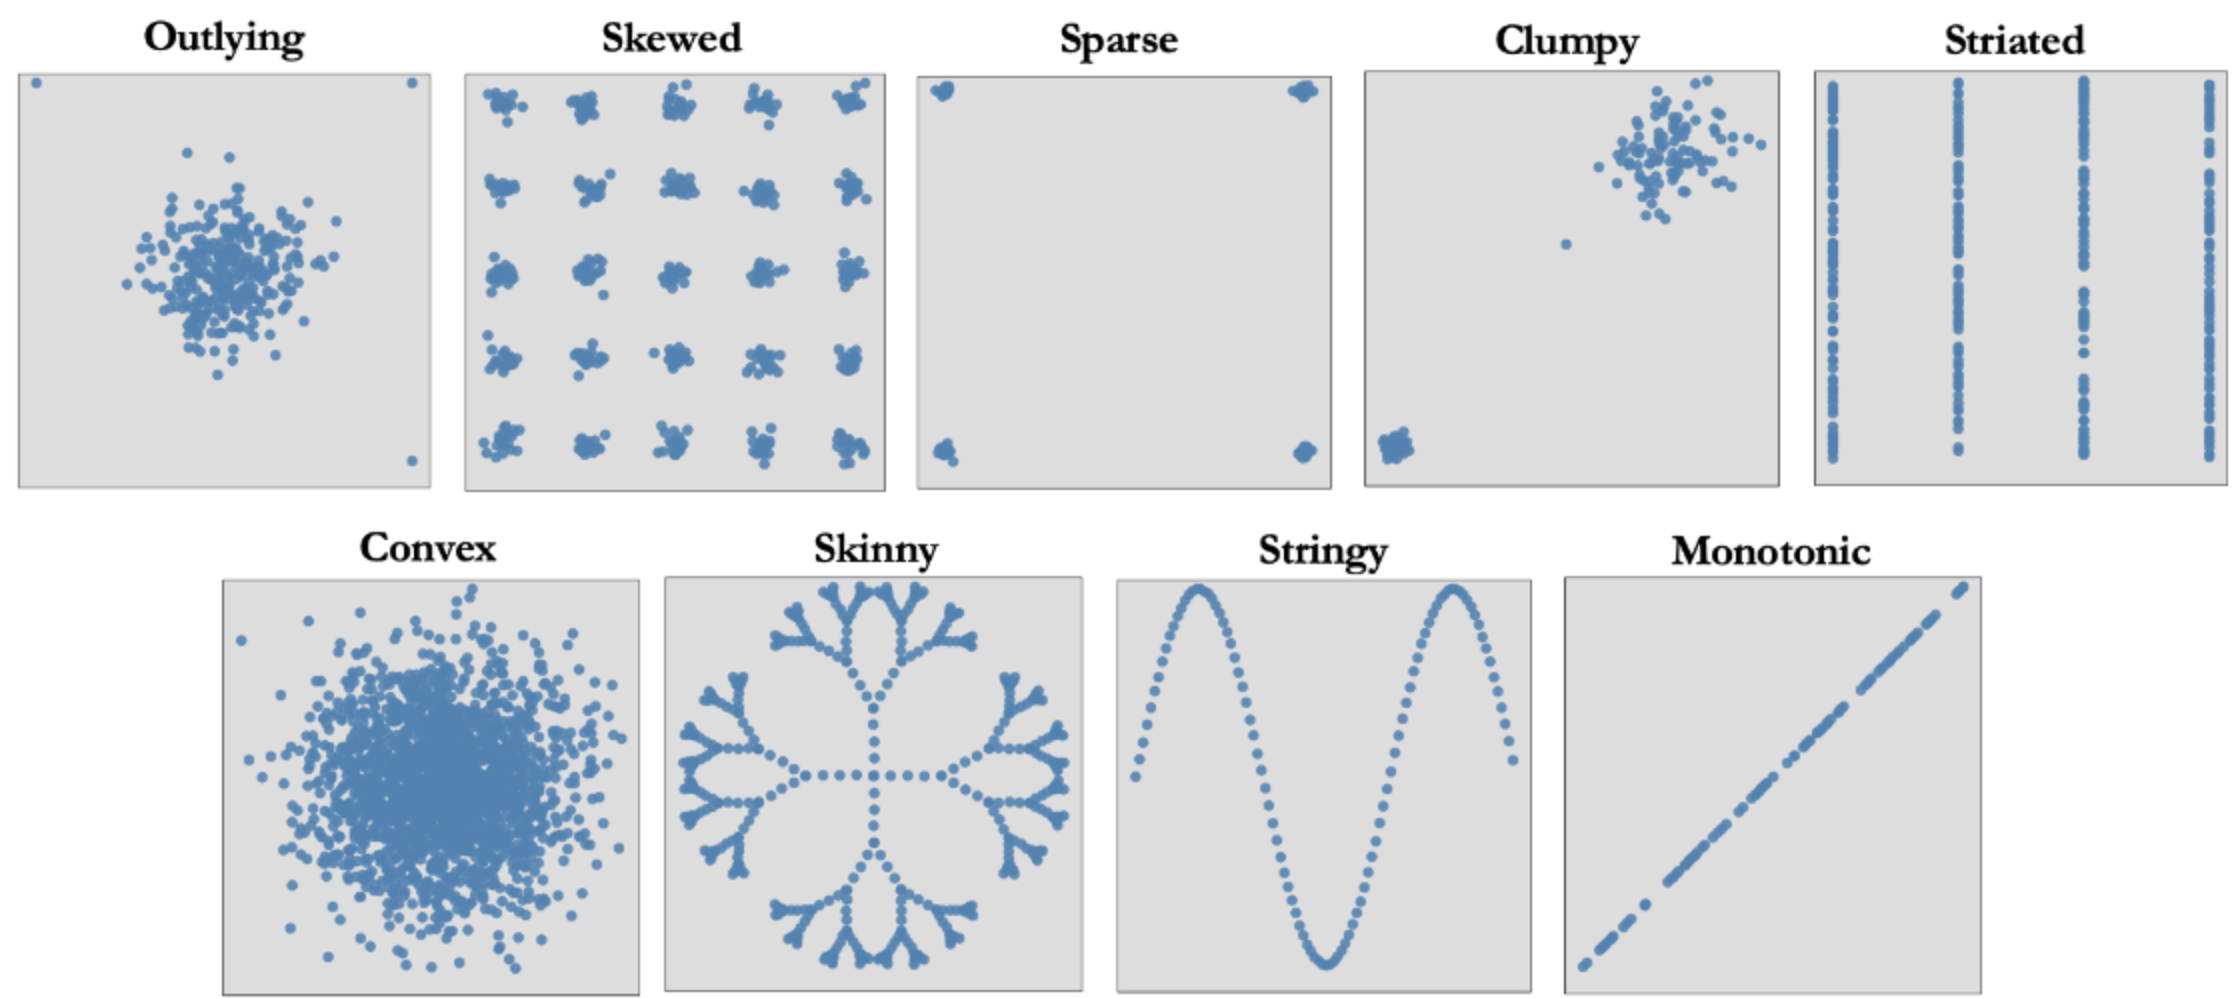
\includegraphics[width=\linewidth]{figs/scagnostics_overview.png}
  \caption{%
  	The nine scagnostics measures, as described in ScagnosticsJS \cite{Wilkie2020}, a JavaScript implementation of graph-theoretic scagnostics ~\cite{Wilkinson2005}. %
  }
  \label{fig:scag_overview}
\end{figure}


% \begin{figure}[tbp]% specify a combination of t, b, p, or h for top, bottom, on its own page, or here
%   \centering % avoid the use of \begin{center}...\end{center} and use \centering instead (more compact)
%   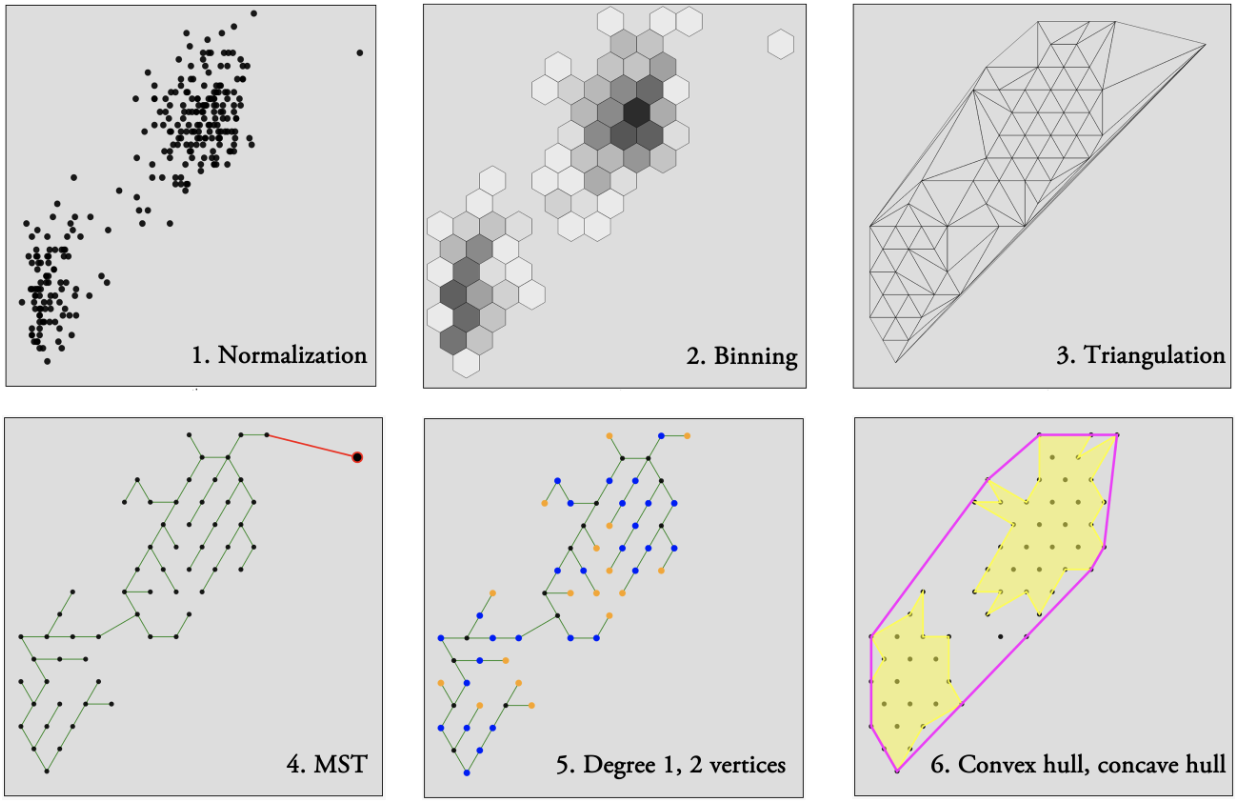
\includegraphics[width=\linewidth]{figs/how_scag_works.png}
%   \caption{%
%   	Computation of graph-theoretic scagnostics, as described in ScanosticsJS \cite{Wilkie2020}. %
%   }
%   \label{fig:how_scag_works}
% \end{figure}

\subsection{Why scagnostics?}
Utility or effectiveness is often quantitatively evaluated by measuring how accurately users can complete a task using the provided visualizations \cite{Elmqvist2012}. Regarding scatterplots, Sarikaya \cite{Sarikaya2018} related the ability to perform scatterplot tasks to the characteristics of the data distribution.

\par For example, take the task of cluster identification. The ability to perform this task depends on the extent to which the data groups into \textbf{clusters}\cite{Sarikaya2018}. This extent can be measured quantitatively using the \textit{clumpy} scagnostic measure. Hence, the difference in the \textit{clumpiness} of the original and privatized data can be a proxy for how much visual utility is preserved by the DP mechanism. If the analyst is to identify clusters on the privatized data, then this difference should be minimized by the DP mechanism. 
\par
This granularity that scagnostics offers in data distribution characteristics makes it suitable to measure visual utility in a task-dependent manner.


\section{Methods}

We hypothesise that scagnostics is a reliable measure of visual utility for differentially private scatterplots. This means we expect the utility to follow certain trends, such as for higher epsilon, the utility must be higher. Moreover, to ensure reliability, the appearance of the data measured by scagnostics must align with the appearance perceived by the user. \par The outputs of differential privacy mechanisms have two characteristics that do not work well with scagnostics - they are binned histograms and tend to be noisy. To overcome these, we implemented two techniques described in sections 4.1 and 4.2.
          
\subsection{Unbinning}
Since scagnostics cannot be applied directly on binned scatterplots, we unbinned them by taking each bin's value $b$ (i.e. the number of points in the bin), and dispersing $b$ points into random positions within the area of the bin. In our testing, the unbinned plots were visually coherent with the binned plots, and the unbinning served as the first step before measuring their appearance with scagnostics.

\subsection{Denoising}
In our testing, we found that scagnostics are \textbf{highly sensitive to noise}. \textcolor{red}{ADD EXAMPLE FOR SENSITIVITY} This was a challenge since adding noise is fundamental to DP mechanisms, and it is something we cannot avoid. To overcome this, we implemented a denoising method - after the DP mechanism is run, only bins with \textit{$\alpha$ or more points} will be unbinned and shown in the final scatterplot, where $\alpha$ is called the \textit{denoise level}.
\par An example is shown in Fig . ~\ref{fig:denoising}. The plot on the top-right is the unbinned version of the DP mechanism's output. Here, we can clearly see that there are 3 clusters despite the noise in between them. But scagnostics cannot make that distinction and thus sees the cluster plus noise as one big clump of data. In contrast, the denoised plot on the bottom right has better separation between the clusters. This aided scagnostics in representing the unbinned plot on the top-right more accurately.


\begin{figure}[tbp]% specify a combination of t, b, p, or h for top, bottom, on its own page, or here
  \centering % avoid the use of \begin{center}...\end{center} and use \centering instead (more compact)
  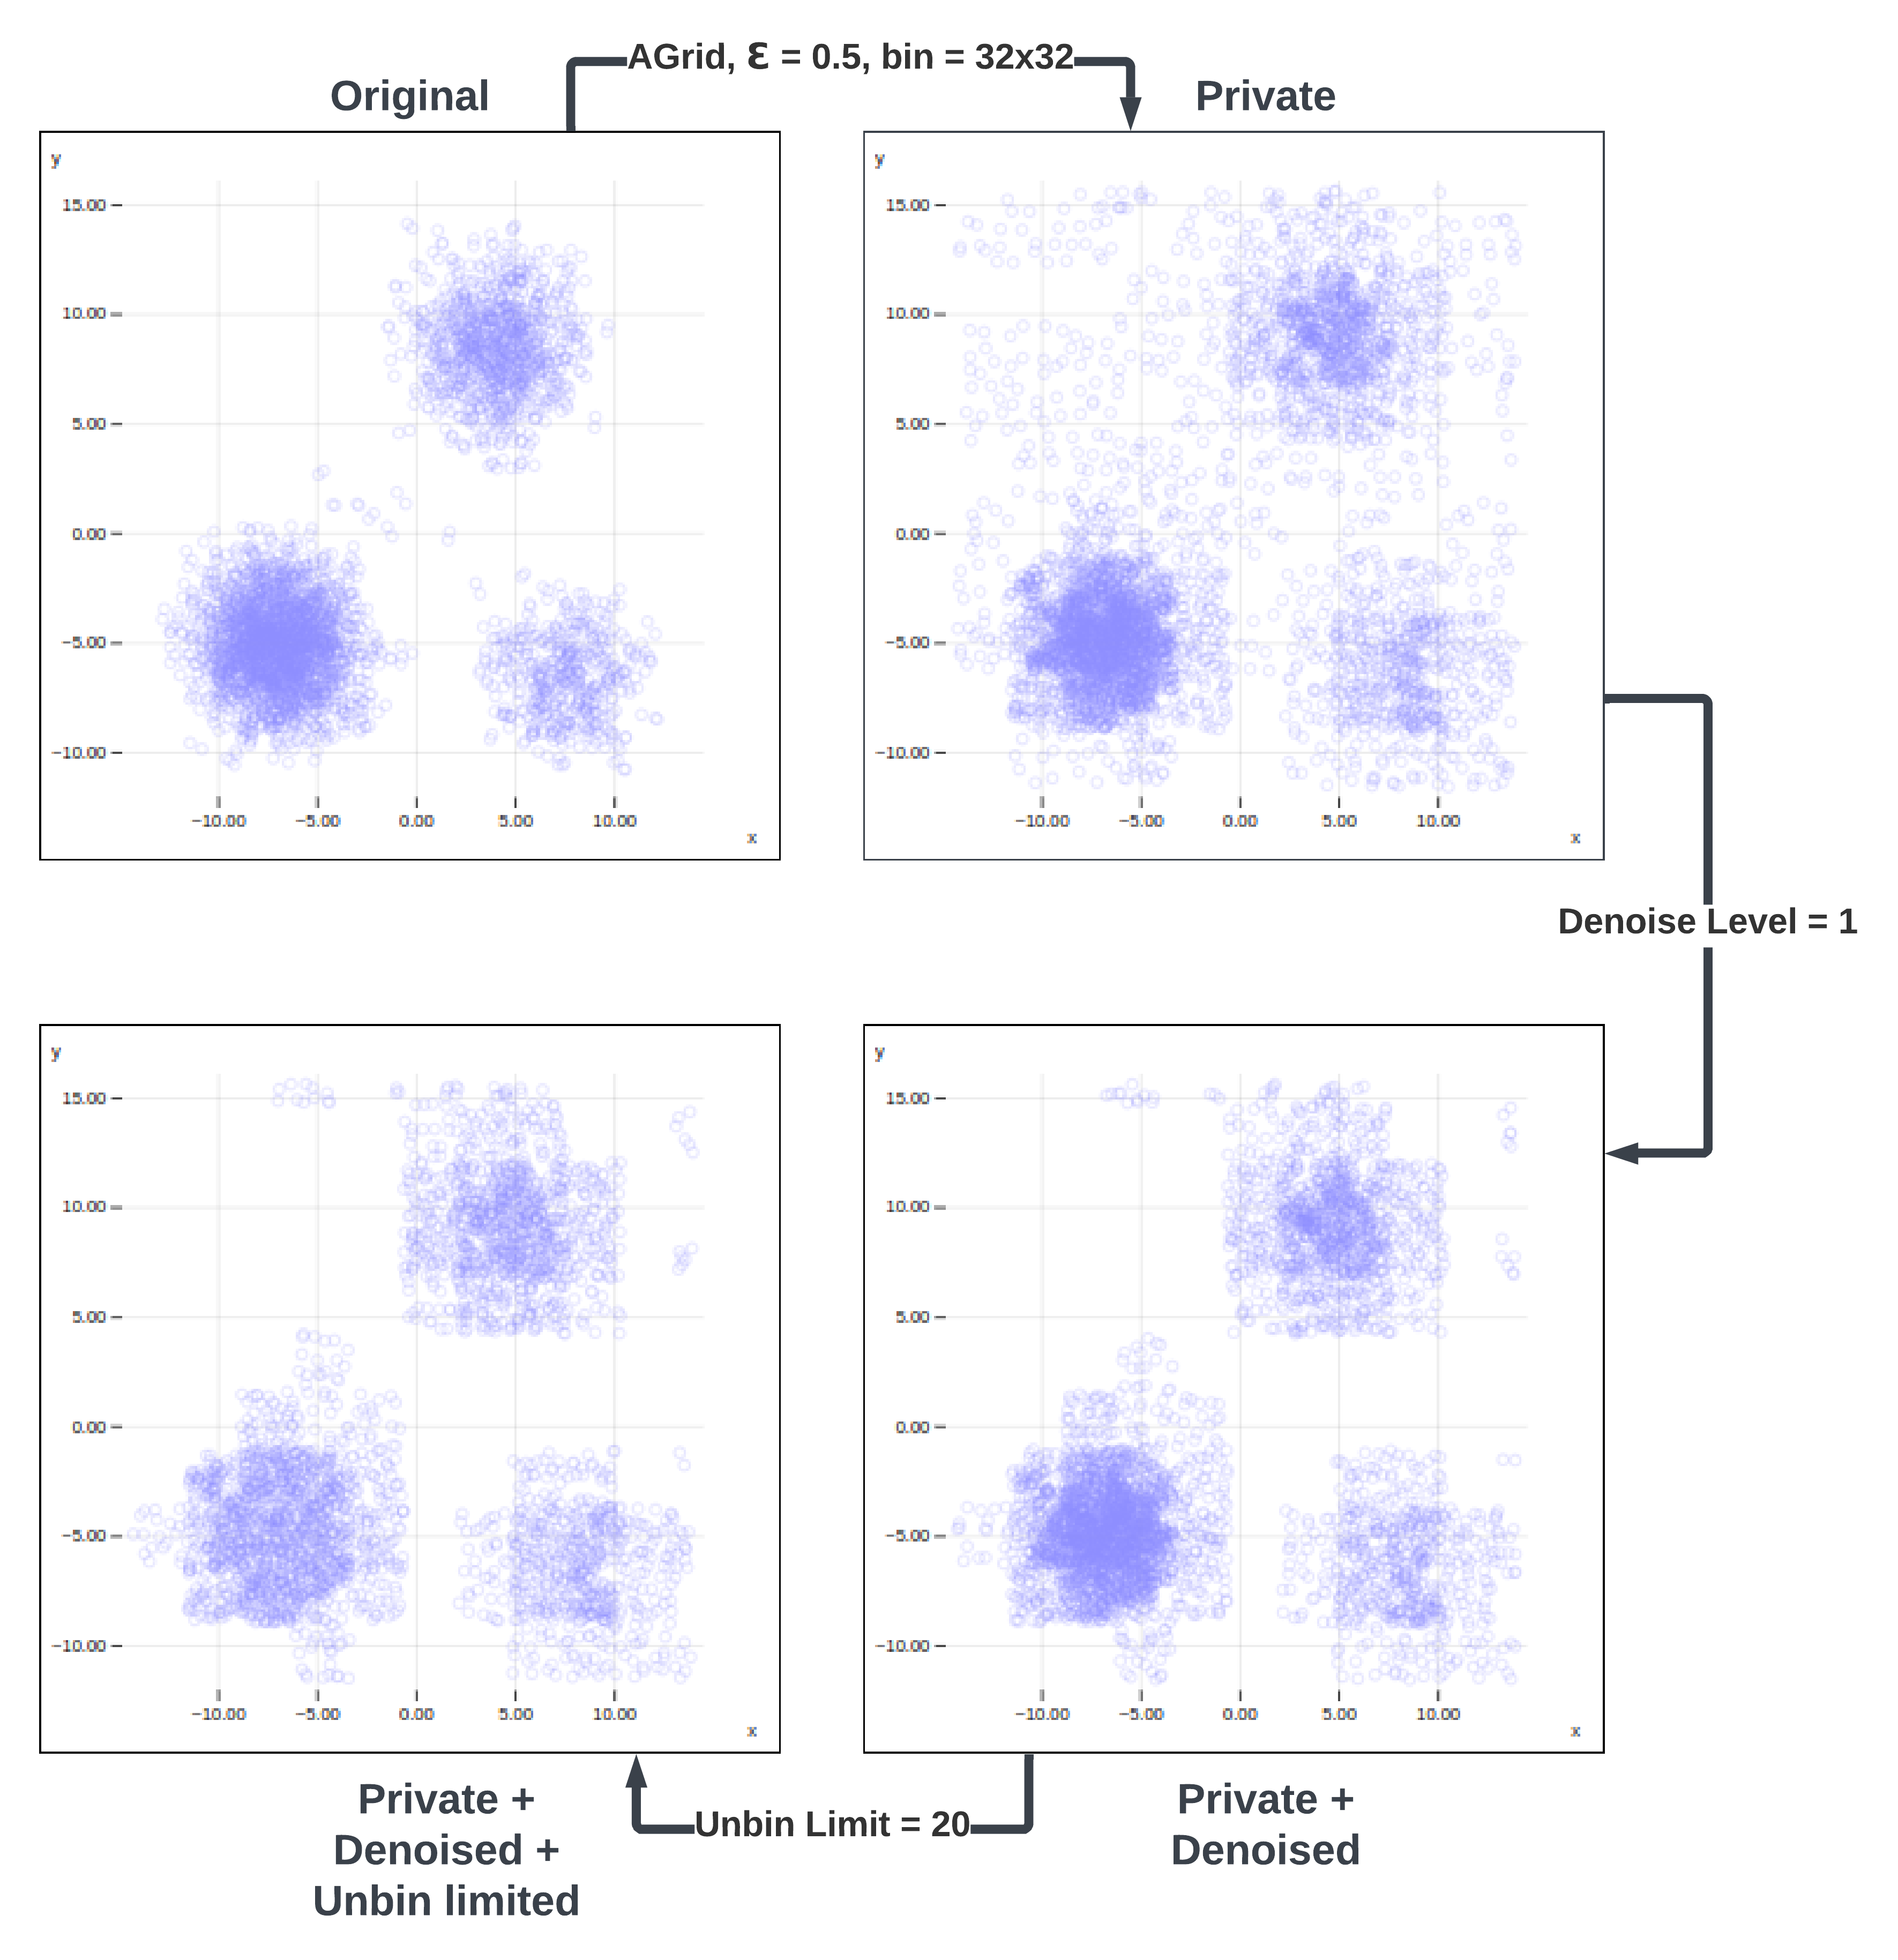
\includegraphics[width=\columnwidth]{figs/denoising + unbinlimit.png}
  \caption{%
  	Effect of denoising to remove sparsely distributed noise. On the left is the unbinned output of AHP on the original data in Figure \ref{fig:the_problem} with $\epsilon=0.5$ and $binning=32x32$, and on the right is the same but without the sparsely distributed noise. This makes Scagnostics to be more representative of what the user perceives. %
  }
  \label{fig:denoising}
\end{figure}

\subsection{Computing visual utility}
To measure the similarity between the original and the privatized plots, \textbf{we mapped each plot to a vector with the 9 scagnostics measures - and calculated the Euclidean distance between the vectors of the original and private data}, denoted as $d_{scag}$. The performance of $d_{scag}$ measure will be discussed in the discussion section. \textcolor{red}{@TODO : Update with actual section}

\subsection{Generating datasets}
We tested this approach on seven synthetic datasets for the original data. Each dataset represented a combination of one or more of the following patterns - clusters, correlations, and striations. These datasets were then privatized with five different DP mechanisms - Laplace mechanism \cite{Dwork2006}, DAWA \cite{li2014}, AHP \cite{Zhang2014}, AGrid \cite{Li2013} and Geometric truncated \cite{Ghosh2009}. The following were the parameters of each DP mechanism, with their possible values:
\begin{itemize}
    \item Epsilon : 0.01, 0.05, 0.1, 0.5
    \item Binning : 32x32, 64x64
\end{itemize}
This gave a total of 280 possible scatterplots from the DP mechanisms. We applied scagnostics on these as well as their denoised versions, coming to a \textbf{grand total of 560 scatterplots. }

\section{Results and discussion}
We measured the $d_{scag}$ and individual scagnostics for all 560 outputs. We will first discuss the performance of $d_{scag}$, and then discuss the ability of individual scagnostics measures to capture the appearance of the scatterplots.

\subsection{Scagnostics as a similarity measure}

\begin{figure}[h]% specify a combination of t, b, p, or h for top, bottom, on its own page, or here
  \centering % avoid the use of \begin{center}...\end{center} and use \centering instead (more compact)
  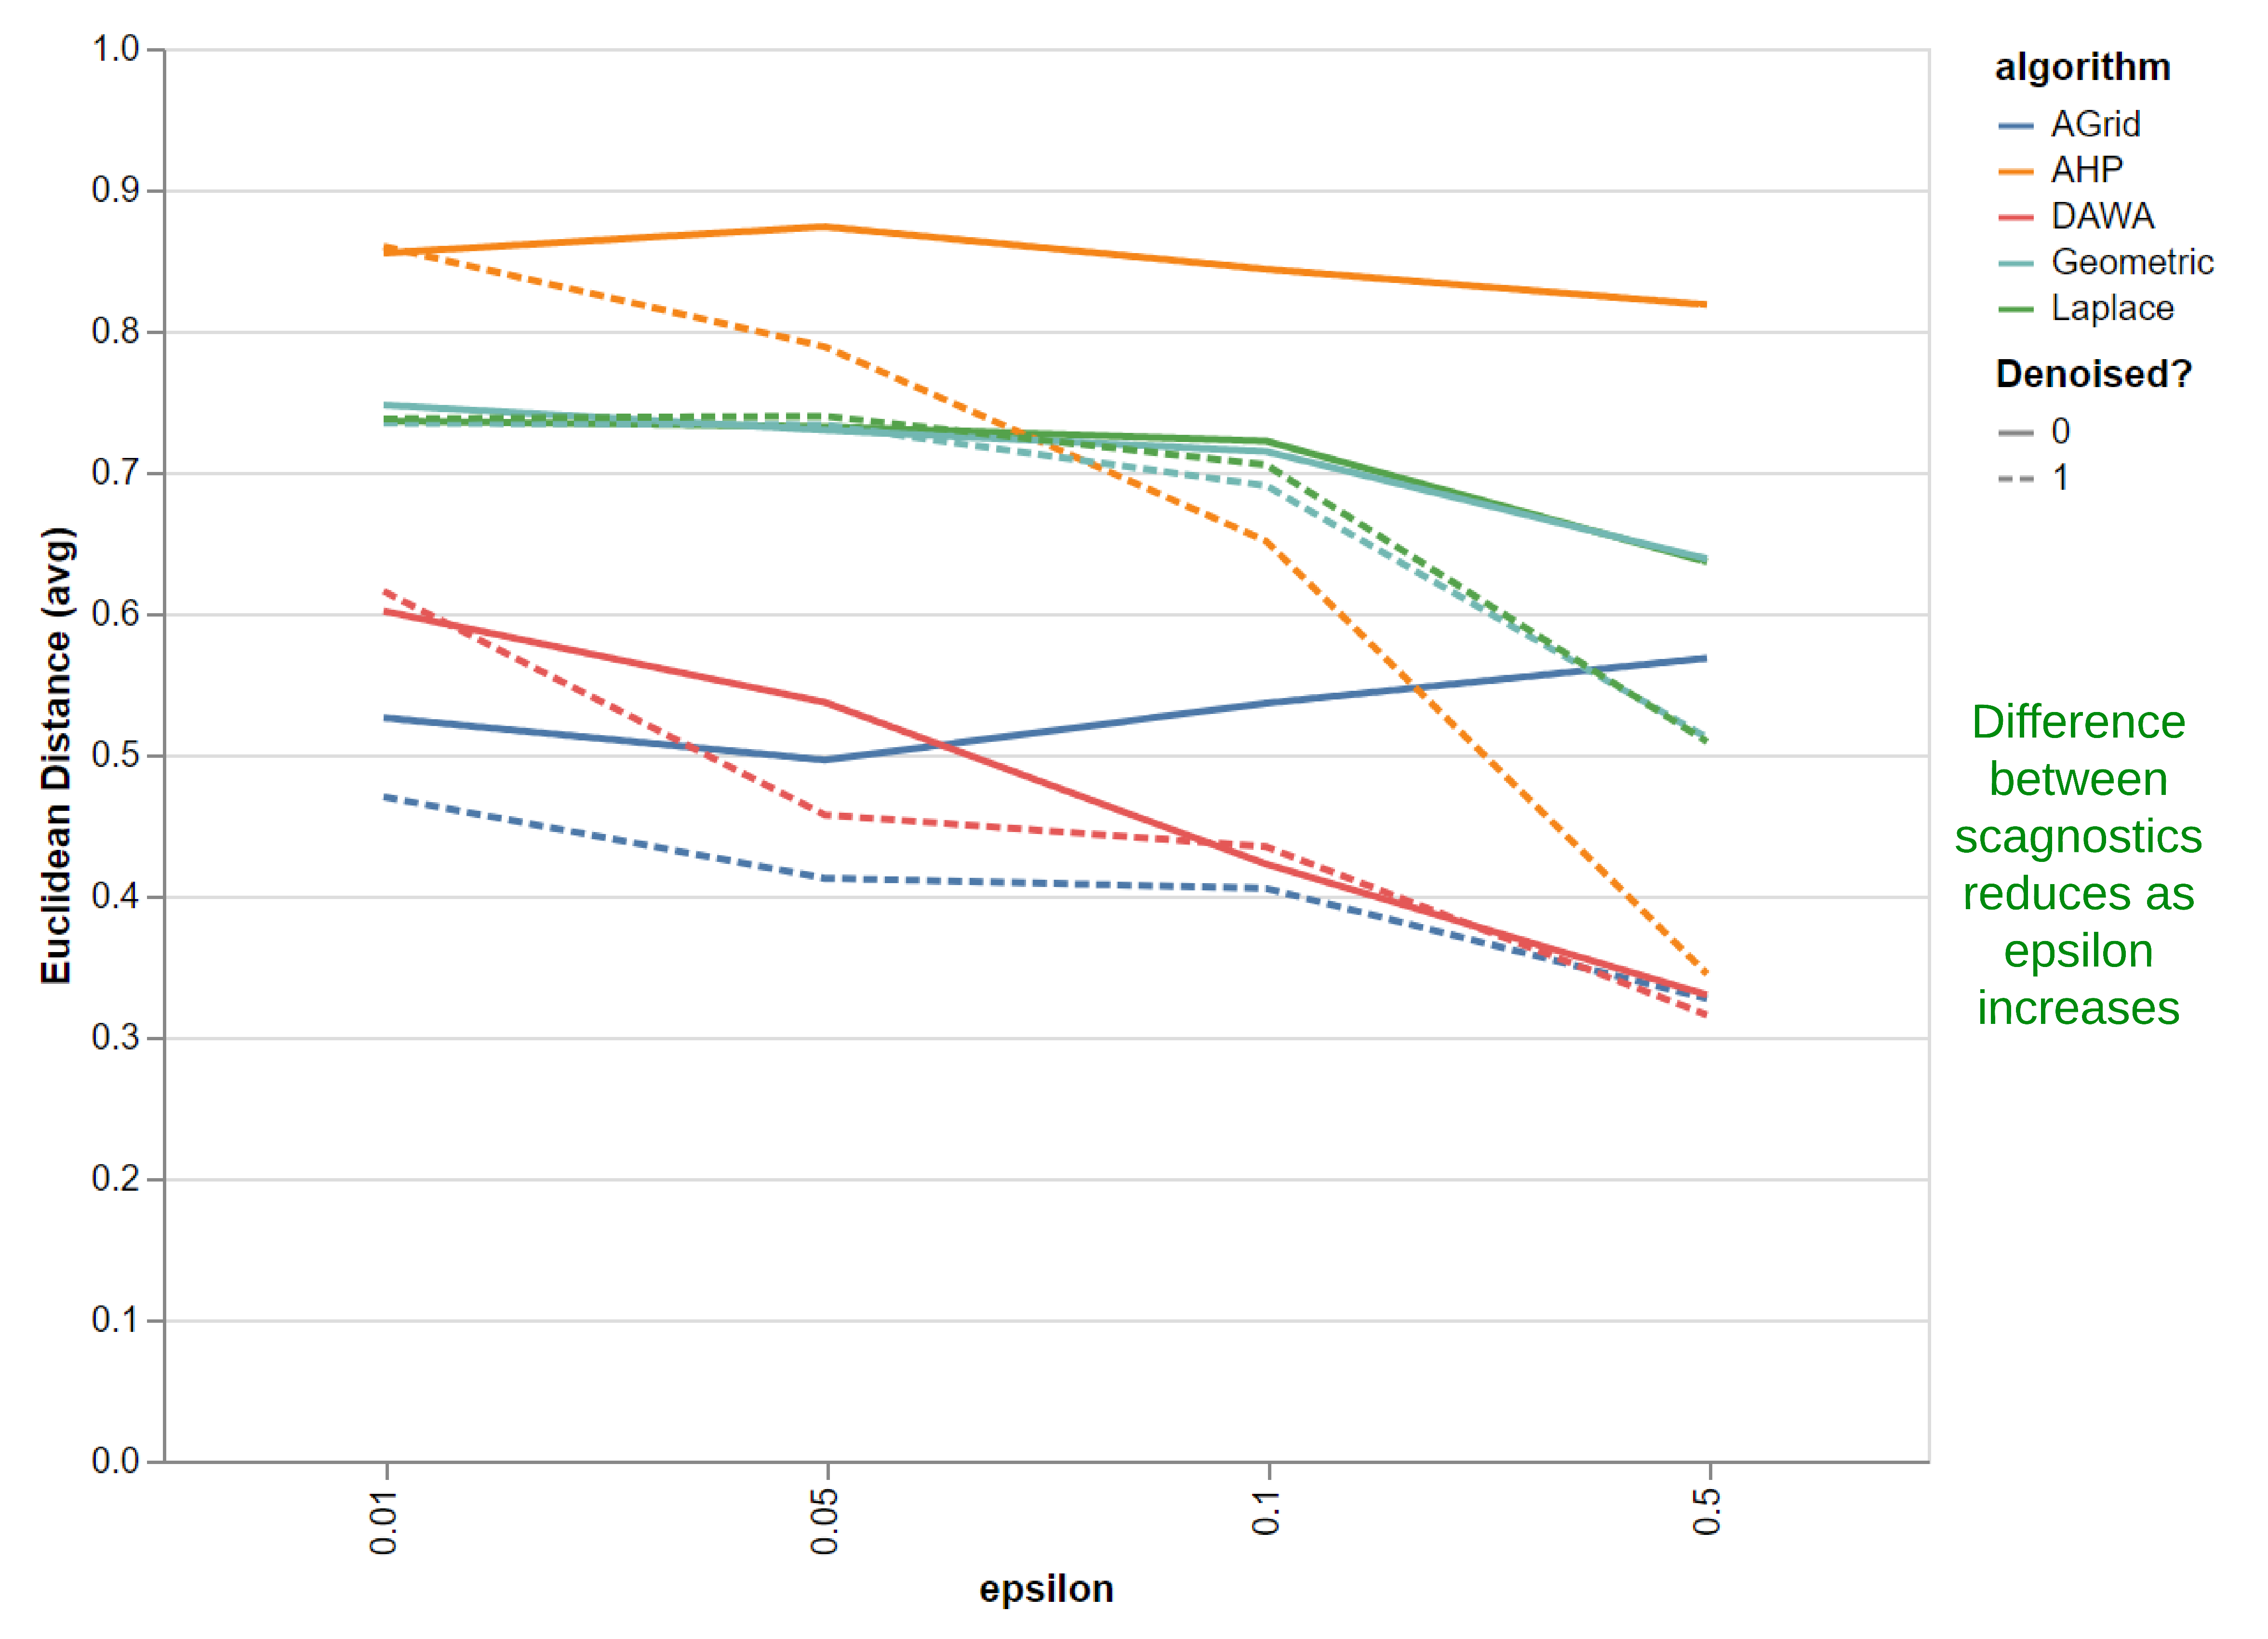
\includegraphics[width=\linewidth]{figs/Score diff reducing with Epsilon.png}
  \caption{%
  	Variance of scagnostics based visual utility with epsilon ($\epsilon$). The higher the $\epsilon$, the lower the amount of noise added to the original data. We observed that the Euclidean distance between scagnostics of the original and privatized plots reduced as $\epsilon$ increased. Moreover, the distance was further reduced when scagnostics were computed on the denoised plots, represented by the dotted lines.%
  }
  \label{fig:diff_reducing_with_epsilon} 
\end{figure}
Fig ~\ref{fig:diff_reducing_with_epsilon} shows the variance of $d_{scag}$ with ($\epsilon$). The higher the value of $d_{scag}$, the lower the visual utility. Overall, the \textbf{reduction of $d_{scag}$ with increasing $\epsilon$} helped validate $d_{scag}$ as a viable measure of visual dissimilarity.
\par We also observed that denoising helped some algorithms more than others. For example, the highest difference in scores due to denoising was shown for plots privatised using AHP, while the lowest difference was for those by the Laplace mechanism. Overall, the denoising helped bring the measures closer to what we perceived visually. However, when using scagnostics individually to capture specific patterns, such as clumpiness, we noticed some inconsistencies in its performance.

\subsection{Measuring appearance}

\begin{figure}[tbp]% specify a combination of t, b, p, or h for top, bottom, on its own page, or here
  \centering % avoid the use of \begin{center}...\end{center} and use \centering instead (more compact)
  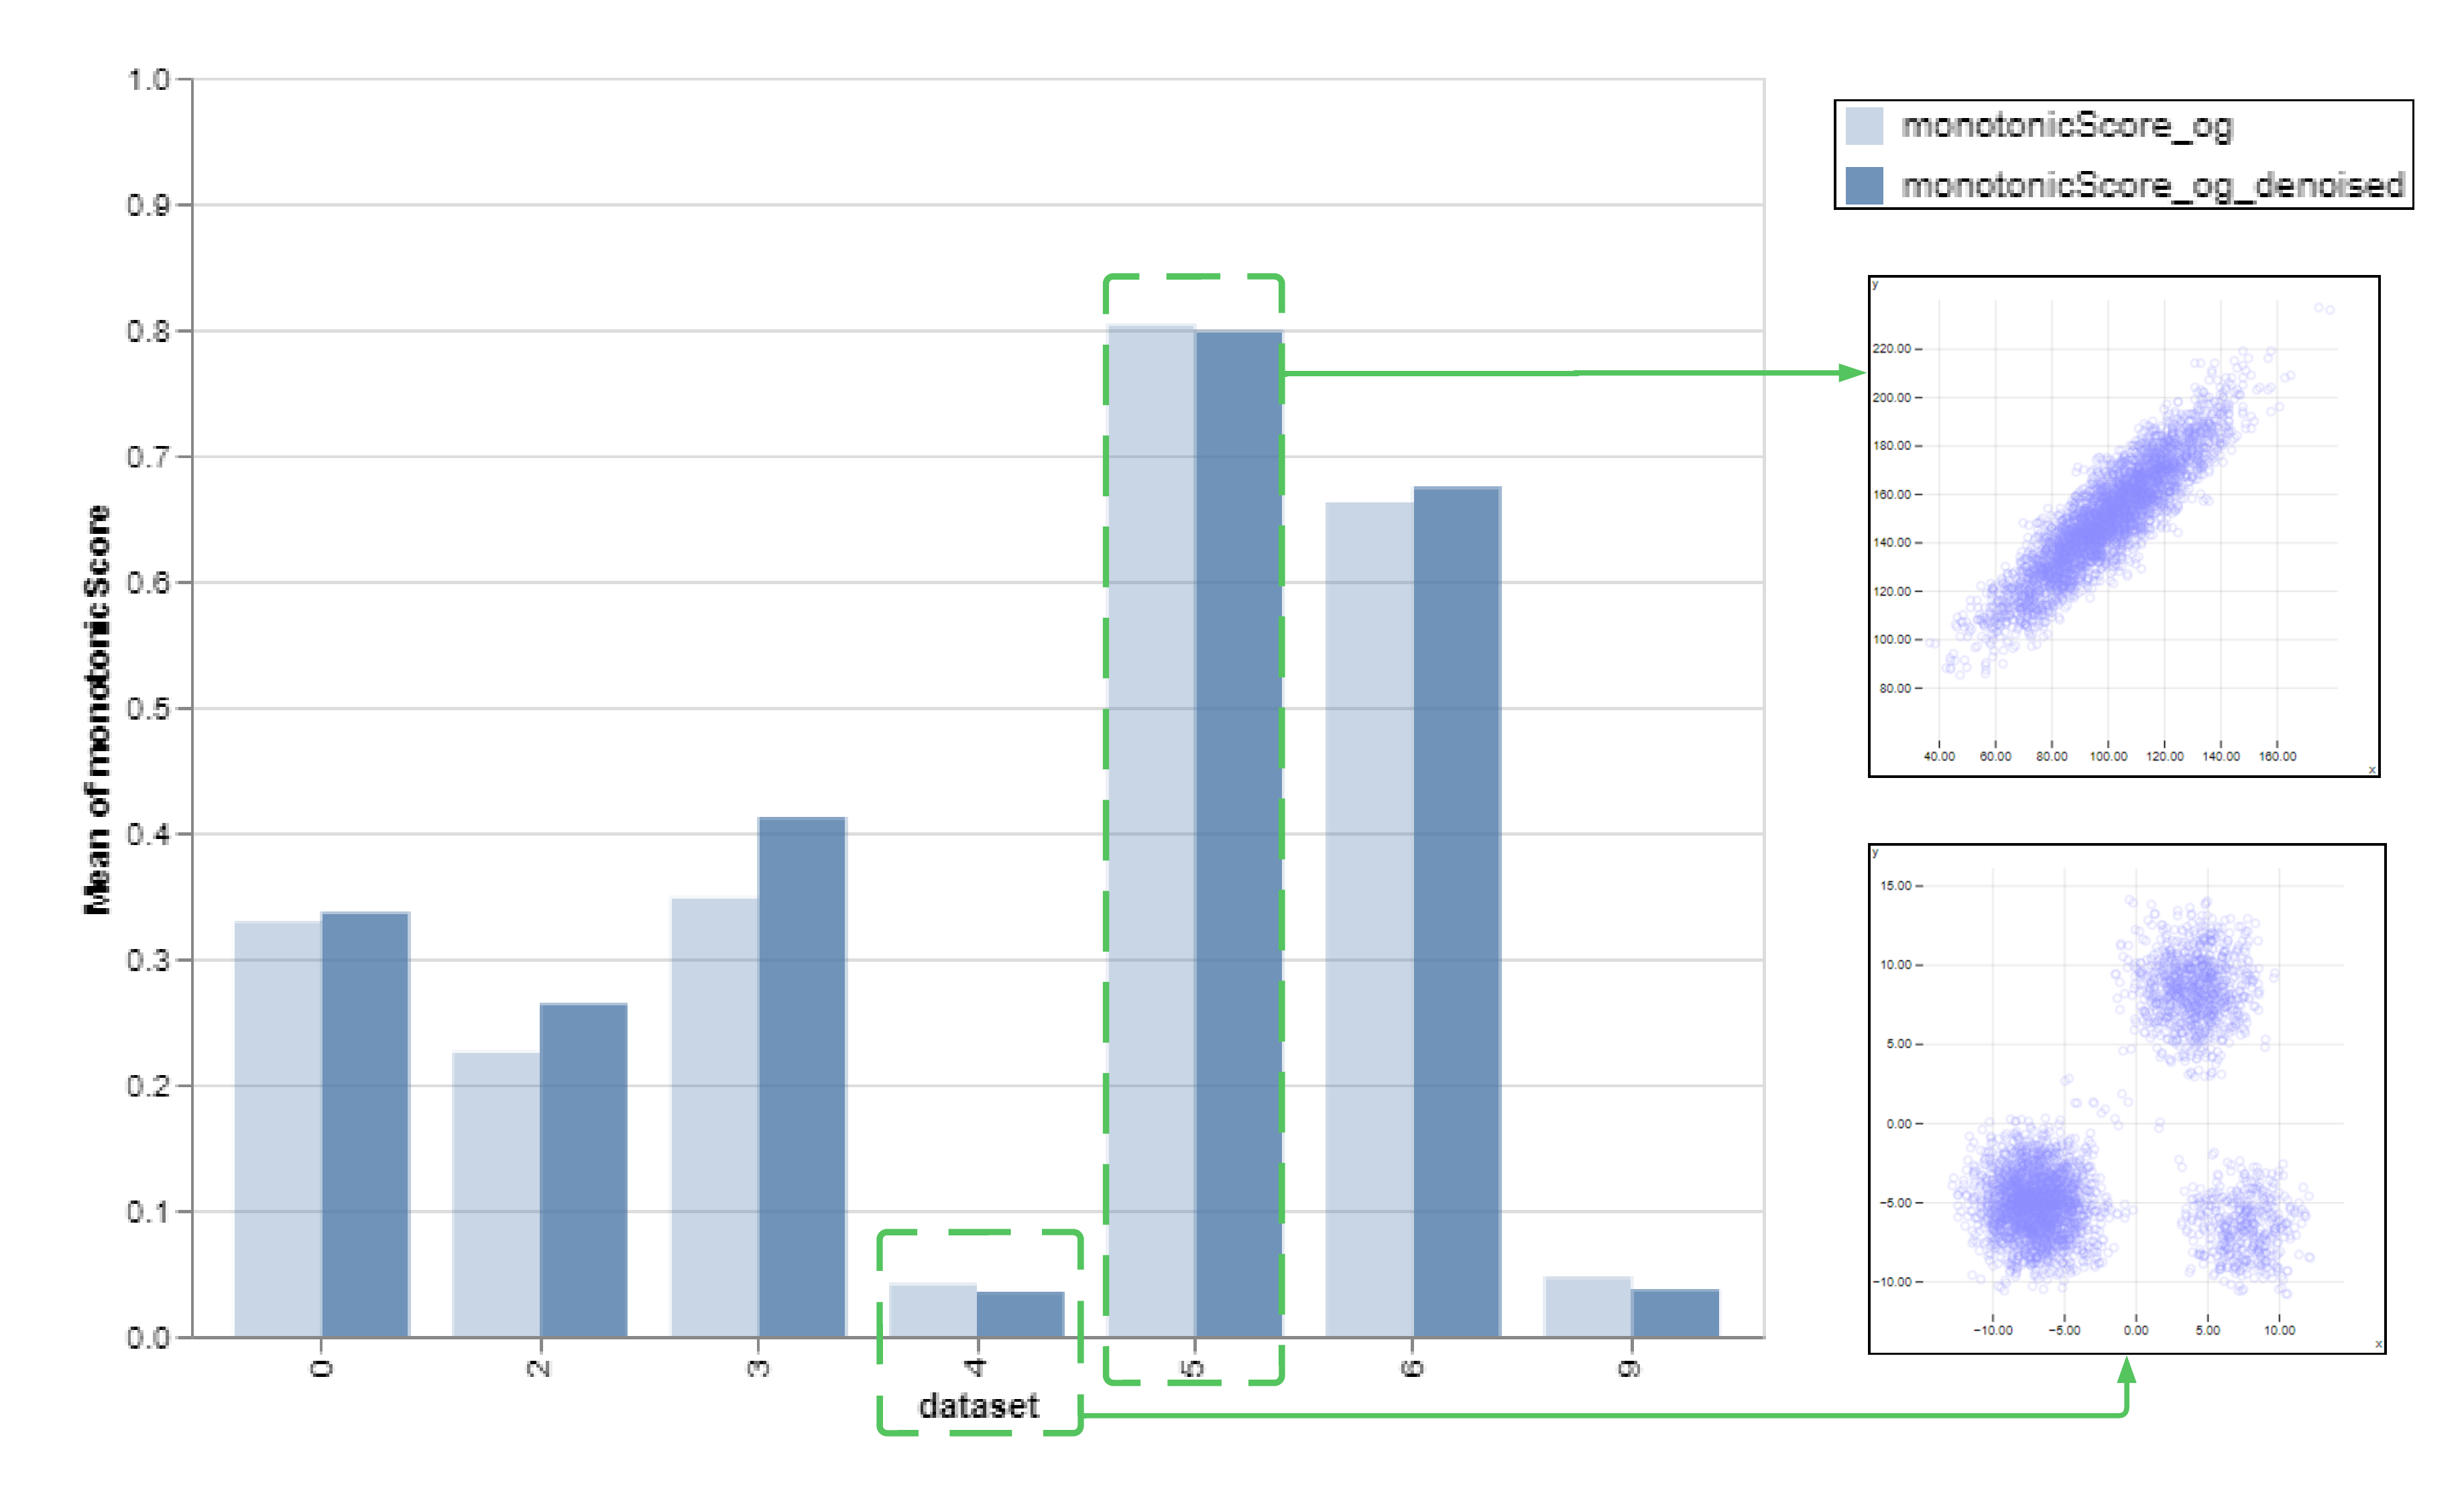
\includegraphics[width=\linewidth]{figs/monotonic_score_as_expected.png}
  \caption{%
  	Monotonic score aligned best with what users see %
  }
  \label{fig:monotonic_score}
\end{figure}

\begin{figure}[tbp]% specify a combination of t, b, p, or h for top, bottom, on its own page, or here
  \centering % avoid the use of \begin{center}...\end{center} and use \centering instead (more compact)
  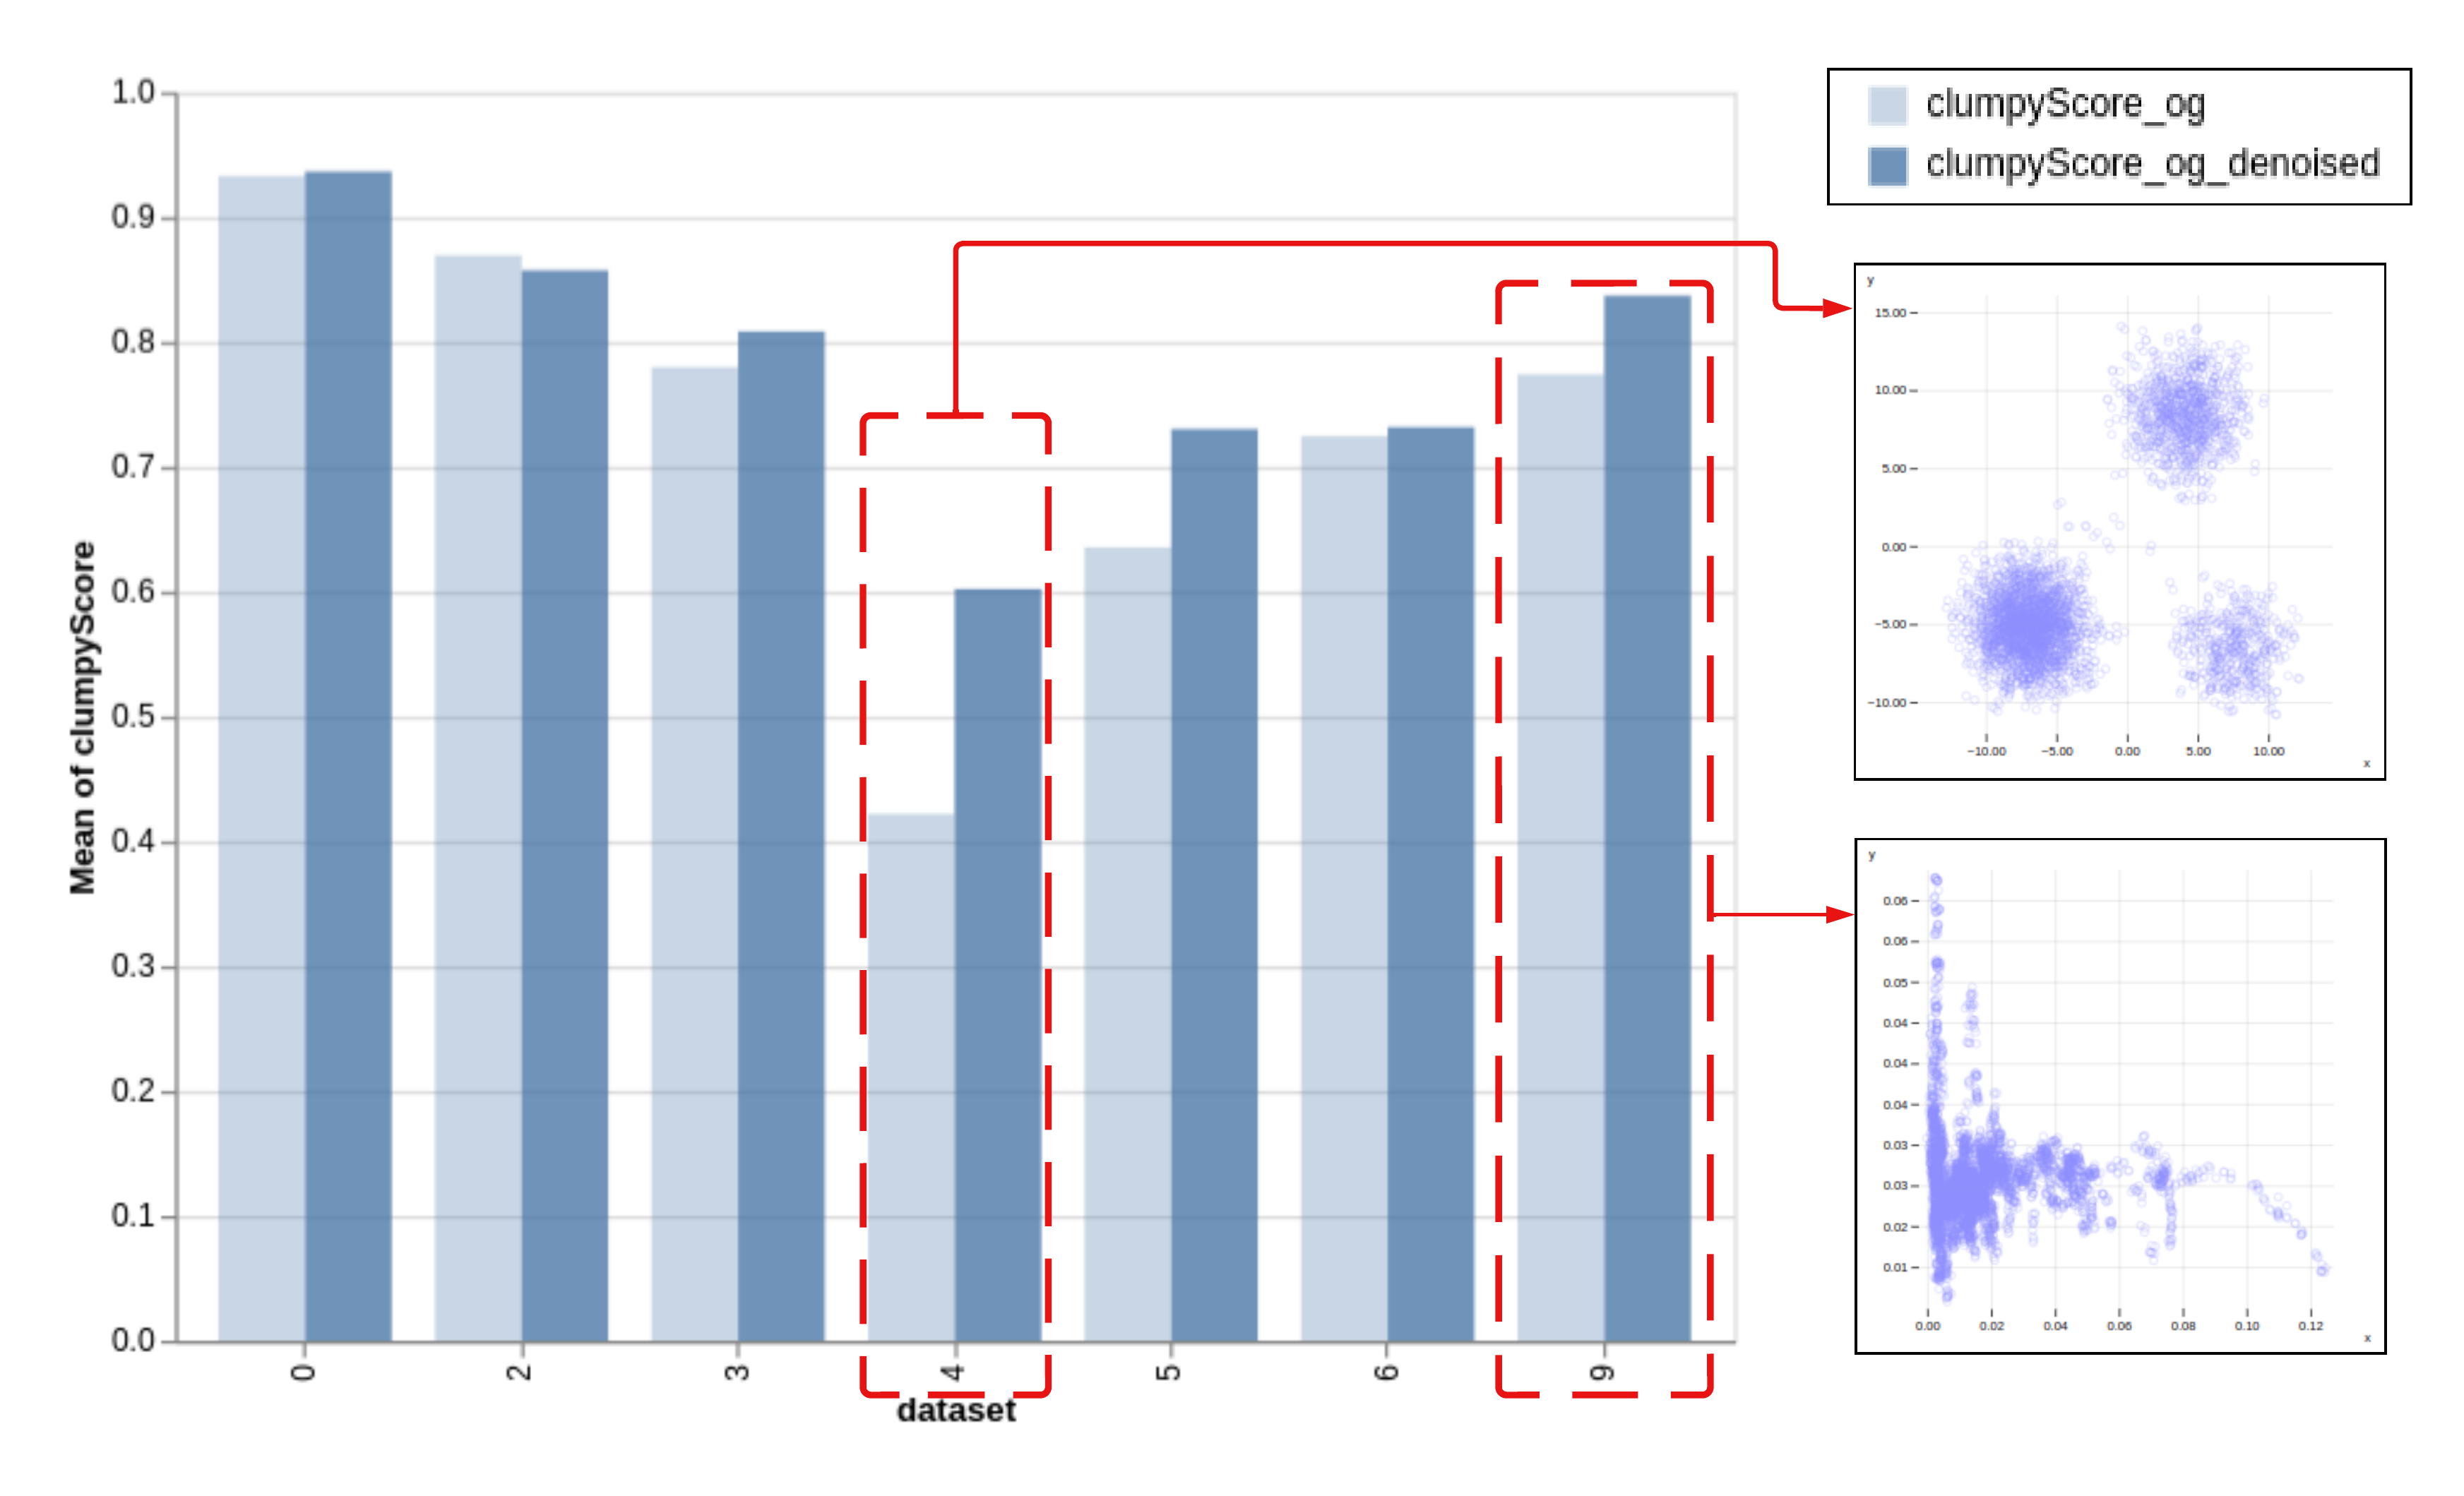
\includegraphics[width=\linewidth]{figs/disparity_of_scagnostics.png}
  \caption{%
  	Disparity between what the users see and \textit{clumpiness} measure. %
  }
  \label{fig:clumpy_score_disparity}
\end{figure}
We observed that scagnostics capture certain patterns much better than others. For example, Figure ~\ref{fig:monotonic_score} shows that the \textit{monotonic} score captured correlated patterns quite effectively. Out of seven, only two datasets exhibited a strong monotonicity pattern which coincides with what the scagnostics measured. However, in \ref{fig:clumpy_score_disparity}, where dataset 4 clearly has three clusters or clumps of data, the \textit{clumpiness} measure was the lowest for this dataset, compared to other plots where cluster formation was not as obvious.  We noticed a similar disparity for the \textit{stringiness} and \textit{skewedness} metrics as well.

\subsection{Re-run with robust Scagnostics}
In addition to the original scagnostics measures by Wilkinson et. al. ~\cite{Wilkinson2005}, we also measured a more robust set of scagnostics proposed by Wang et al. ~\cite{Wang2020}. They improved on Wilkinson's original work by :
\begin{itemize}
    \item Reducing the sensitivity of scagnostics to noise
    \item Measuring human perception of \textit{clumpiness} through a user study
    \item Modifying the \textit{clumpiness} measure to align towards the human perception of clumpiness
\end{itemize}

\subsection{Limitations}
This work clarifies the performance of scagnostics in measuring visual utility. However, we have not collected data on how \textit{humans} perceive the visual utility of differentially private scatterplots. An outcome of a user study would be a ranking of privatized plots based on utility. We would then check if the ranking obtained from scagnostics matched the ranking from the study. Such a method would then provide more validity to our metric of visual utility.

\textbf{Edit - July 10th, 2023:} Panavas et. al. \cite{Panavas2023} recently conducted a user study which asked visualization experts to rate the visual utility of differentially private plots. Additionally, they measured utility using five automated measures - one of which was scagnostics - and compared their rankings of the plot to the ranking concluded from the study. They found that scagnostics had\textit{ the lowest correlation} to the notion of visual utility as perceived by humans. With this project, we have dug deeper into that result by analyzing the effects of denoising and unbinning thresholds on scagnostics and also trying robust scagnostics.


\section{Conclusion and Future work}
Measuring utility in any context is not an easy task. For the visual context, we have demonstrated that scagnostics have the potential to measure visual utility. However, they are not perfect, and we found inconsistencies between what scagnostics claimed to measure and what we found in our testing. This opens a new direction to discover why these inconsistencies occur and whether they are solvable.





% You should specify ORCID IDs for each author (see \url{https://orcid.org/}  to register) for disambiguation and long-term contact preservation.
% Use \verb|\authororcid{Author Name}{0000-0000-0000-0000}| for each author, replacing the ``Author Name'' and using the 16-digit (hyphenated) ORCID ID for the second parameter.
% The template shows an example without ORCID IDs for two of the authors.
% ORCID IDs should be provided in all cases.

% Each author's affiliations have to be provided in the author footer on the bottom-left corner of the first page.
% It is permitted to merge two or more people from the same institution as long as they are shown in the same order as in the overall author sequence on the top of the first page.
% For example, if authors A, B, C, and D are from institutions 1, 2, 1, and 2, respectively, then it is ok to use 2 bullets as follows:
% \begin{itemize}
%   \item A and C are with Institution 1. E-mail: \{a\,$|$\,c\}@i1.com\,.

%   \item B and D are with Institution 2. E-mail: \{b\,$|$\,d\}@i2.org\,.
% \end{itemize}


% \begin{table}[tb]
%   \caption{%
%   	VIS/VisWeek accepted/presented papers: 1990--2016.%
%   }
%   \label{tab:vis_papers}
%   \scriptsize%
%   \centering%
%   \begin{tabu}{%
%   	  r%
%   	  	*{7}{c}%
%   	  	*{2}{r}%
%   	}
%   	\toprule
%   	year & \rotatebox{90}{Vis/SciVis} &   \rotatebox{90}{SciVis conf} &   \rotatebox{90}{InfoVis} &   \rotatebox{90}{VAST} &   \rotatebox{90}{VAST conf} &   \rotatebox{90}{TVCG @ VIS} &   \rotatebox{90}{CG\&A @ VIS} &   \rotatebox{90}{VIS/VisWeek} \rotatebox{90}{incl.\ TVCG/CG\&A}   &   \rotatebox{90}{VIS/VisWeek} \rotatebox{90}{w/o TVCG/CG\&A}   \\
%   	\midrule
%   	2016 & 30 &   & 37 & 33 & 15 & 23 & 10 & 148 & 115 \\
%   	2015 & 33 & 9 & 38 & 33 & 14 & 17 & 15 & 159 & 127 \\
%   	2014 & 34 &   & 45 & 33 & 21 & 20 &    & 153 & 133 \\
%   	2013 & 31 &   & 38 & 32 &    & 20 &    & 121 & 101 \\
%   	2012 & 42 &   & 44 & 30 &    & 23 &    & 139 & 116 \\
%   	2011 & 49 &   & 44 & 26 &    & 20 &    & 139 & 119 \\
%   	2010 & 48 &   & 35 & 26 &    &    &    & 109 & 109 \\
%   	2009 & 54 &   & 37 & 26 &    &    &    & 117 & 117 \\
%   	2008 & 50 &   & 28 & 21 &    &    &    &  99 &  99 \\
%   	2007 & 56 &   & 27 & 24 &    &    &    & 107 & 107 \\
%   	2006 & 63 &   & 24 & 26 &    &    &    & 113 & 113 \\
%   	2005 & 88 &   & 31 &    &    &    &    & 119 & 119 \\
%   	2004 & 70 &   & 27 &    &    &    &    &  97 &  97 \\
%   	2003 & 74 &   & 29 &    &    &    &    & 103 & 103 \\
%   	2002 & 78 &   & 23 &    &    &    &    & 101 & 101 \\
%   	2001 & 74 &   & 22 &    &    &    &    &  96 &  96 \\
%   	2000 & 73 &   & 20 &    &    &    &    &  93 &  93 \\
%   	1999 & 69 &   & 19 &    &    &    &    &  88 &  88 \\
%   	1998 & 72 &   & 18 &    &    &    &    &  90 &  90 \\
%   	1997 & 72 &   & 16 &    &    &    &    &  88 &  88 \\
%   	1996 & 65 &   & 12 &    &    &    &    &  77 &  77 \\
%   	1995 & 56 &   & 18 &    &    &    &    &  74 &  74 \\
%   	1994 & 53 &   &    &    &    &    &    &  53 &  53 \\
%   	1993 & 55 &   &    &    &    &    &    &  55 &  55 \\
%   	1992 & 53 &   &    &    &    &    &    &  53 &  53 \\
%   	1991 & 50 &   &    &    &    &    &    &  50 &  50 \\
%   	1990 & 53 &   &    &    &    &    &    &  53 &  53 \\
%   	\midrule               
%   	\textbf{sum} & \textbf{1545} & \textbf{9} & \textbf{632} & \textbf{310} & \textbf{50} & \textbf{123} & \textbf{25} & \textbf{2694} & \textbf{2546} \\
%   	\bottomrule
%   \end{tabu}%
% \end{table}




\section{Supplemental Material Instructions}
\label{sec:supplement_inst}
The code for this project is split into two parts:
\begin{itemize}
    \item A Python notebook for running the differential privacy mechanisms, along with our test datasets. We recommend running the notebook on Google Colab to avoid OS-related compatibility issues \footnote[2]{https://osf.io/xykef/}
    \item GitHub repo of the frontend system shown in Figure \ref{fig:teaser} \footnote[3]{https://github.com/harith1996/dp-utility-scagnostics}
\end{itemize}

\section{References}
\label{sec:references_inst}

An example of the reference formatting is provided in the \textbf{References} section at the end.

%% if specified like this the section will be ommitted in review mode
\acknowledgments{%
	The authors wish to thank A, B, and C.
  This work was supported in part by a grant from XYZ (\# 12345-67890).%
}


\bibliographystyle{abbrv-doi-hyperref}
%\bibliographystyle{abbrv-doi-hyperref-narrow}
%\bibliographystyle{abbrv-doi}
%\bibliographystyle{abbrv-doi-narrow}

\bibliography{template}


\appendix % You can use the `hideappendix` class option to skip everything after \appendix



\end{document}

